% !TeX root = syllabus_ELEC0053.tex
% !TeX encoding = ISO-8859-1
% !TeX spellcheck = fr_FR

\section{Exercices non r�solus}
\begin{exercise}{}
D�terminer l'expression du gain en boucle ferm�e, de l'imp�dance
d'entr�e et de l'imp�dance de sortie du montage
isolateur repr�sent� ci-dessous lorsque :
\begin{enumerate}
	\item le gain en boucle ouverte de l'AO $\quad A=10^5$;
	\item l'imp�dance d'entr�e diff�rentielle de l'AO $\quad Z_i=R_{i}=100$
	k$\Omega$;
	\item l'imp�dance  de sortie de l'AO $\quad Z_o=R_{o}=10\,\,\Omega$;
	\item l'imp�dance  interne de la source $\quad Z_s=R_s=1$ k$\Omega$;
	\item l'imp�dance de charge  $\quad Z_L=R_L=1$ k$\Omega$.
\end{enumerate}
\begin{center}
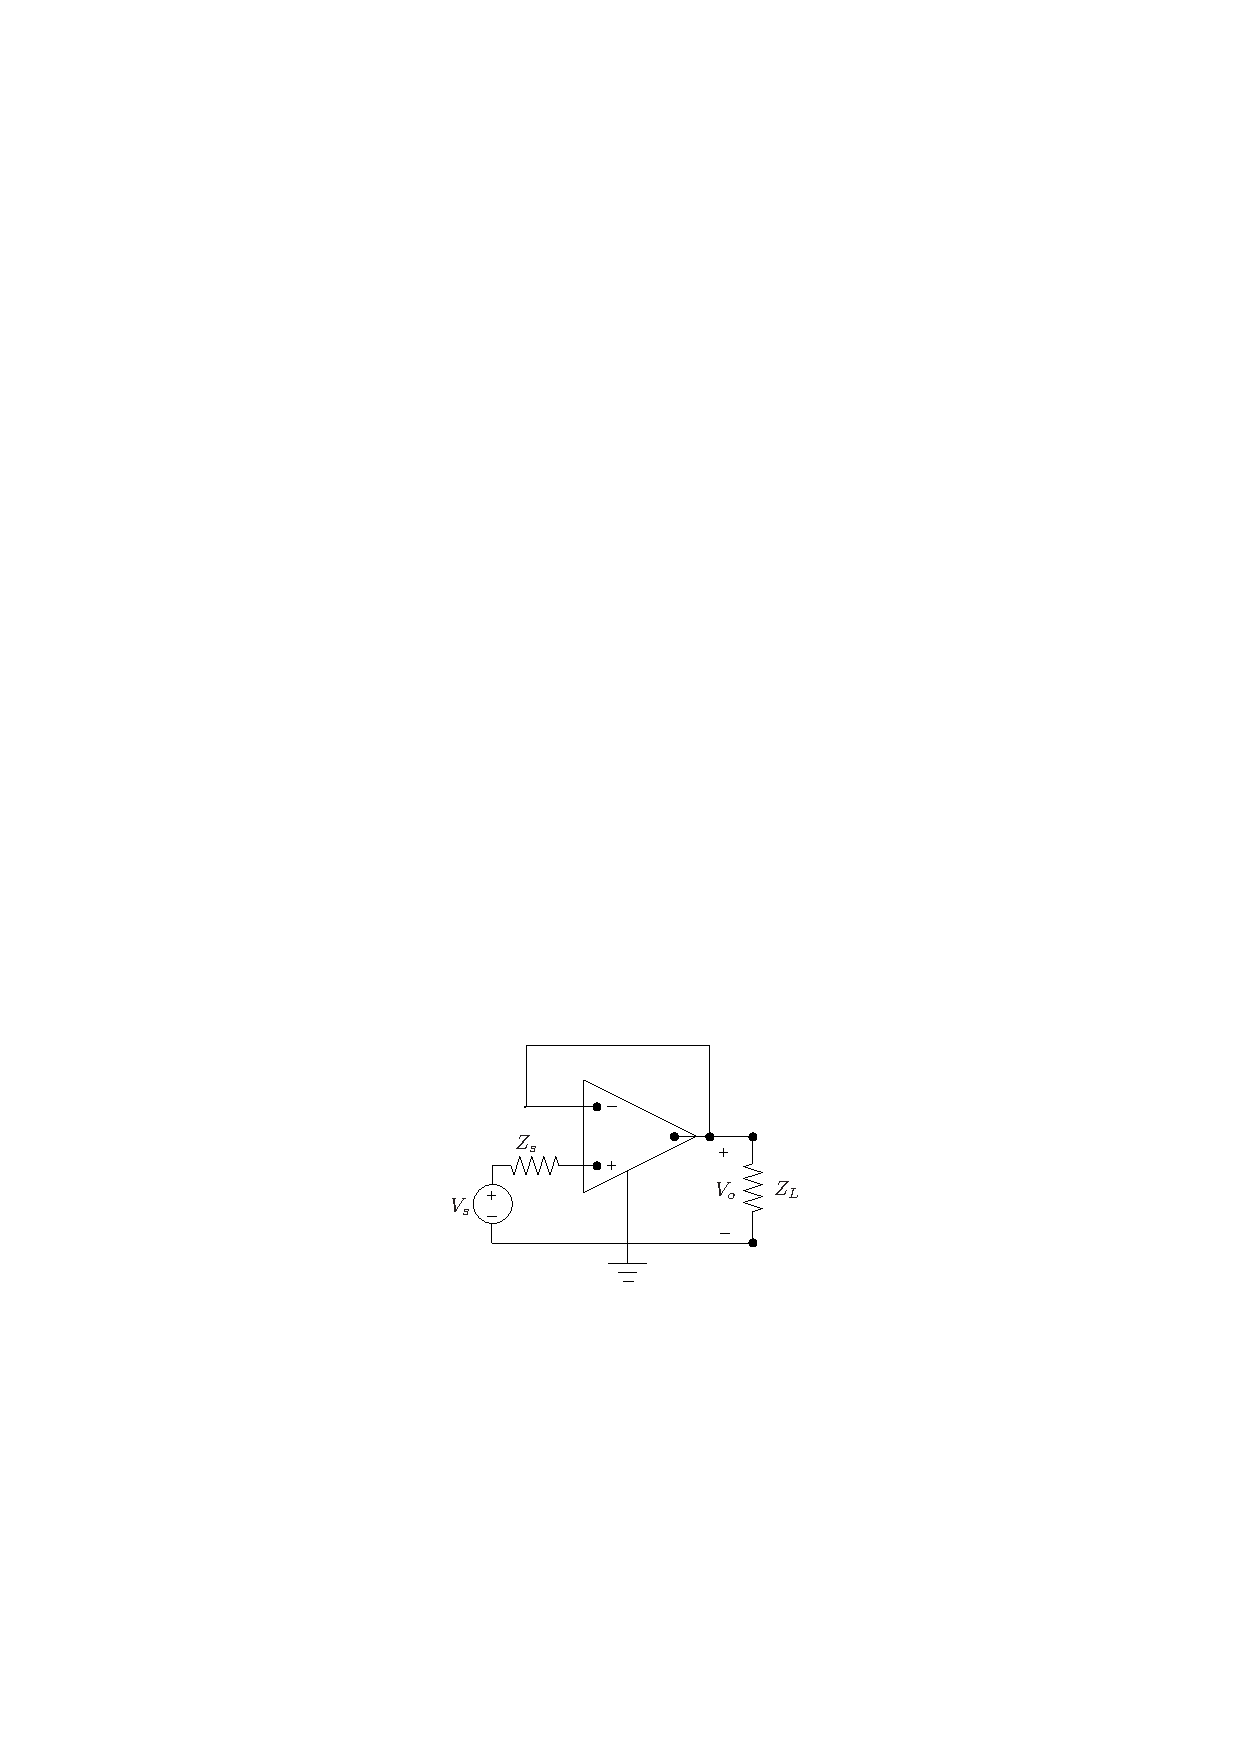
\includegraphics[width=0.6\textwidth]{exercices/ex-4-1}
\end{center}

\rep{$\frac{V_o}{V_i}=\frac{Z_L(Z_o+AZ_i)}{(Z_i+Z_s)(Z_o+Z_L)+Z_L(AZ_i+Z_o)}$\\
	$Z_{in}=Z_i+Z_s+  \frac{Z_o Z_L}{Z_o+Z_L}\left( 1+A\frac{Z_i}{Z_o}\right)$\\
	$Z_{out}= \frac{Z_o(Z_i+Z_s)}{Z_o+Z_s+(1+A)Z_i}$}
\end{exercise}

\begin{exercise}{}
On consid�re le circuit suivant
\begin{center}
	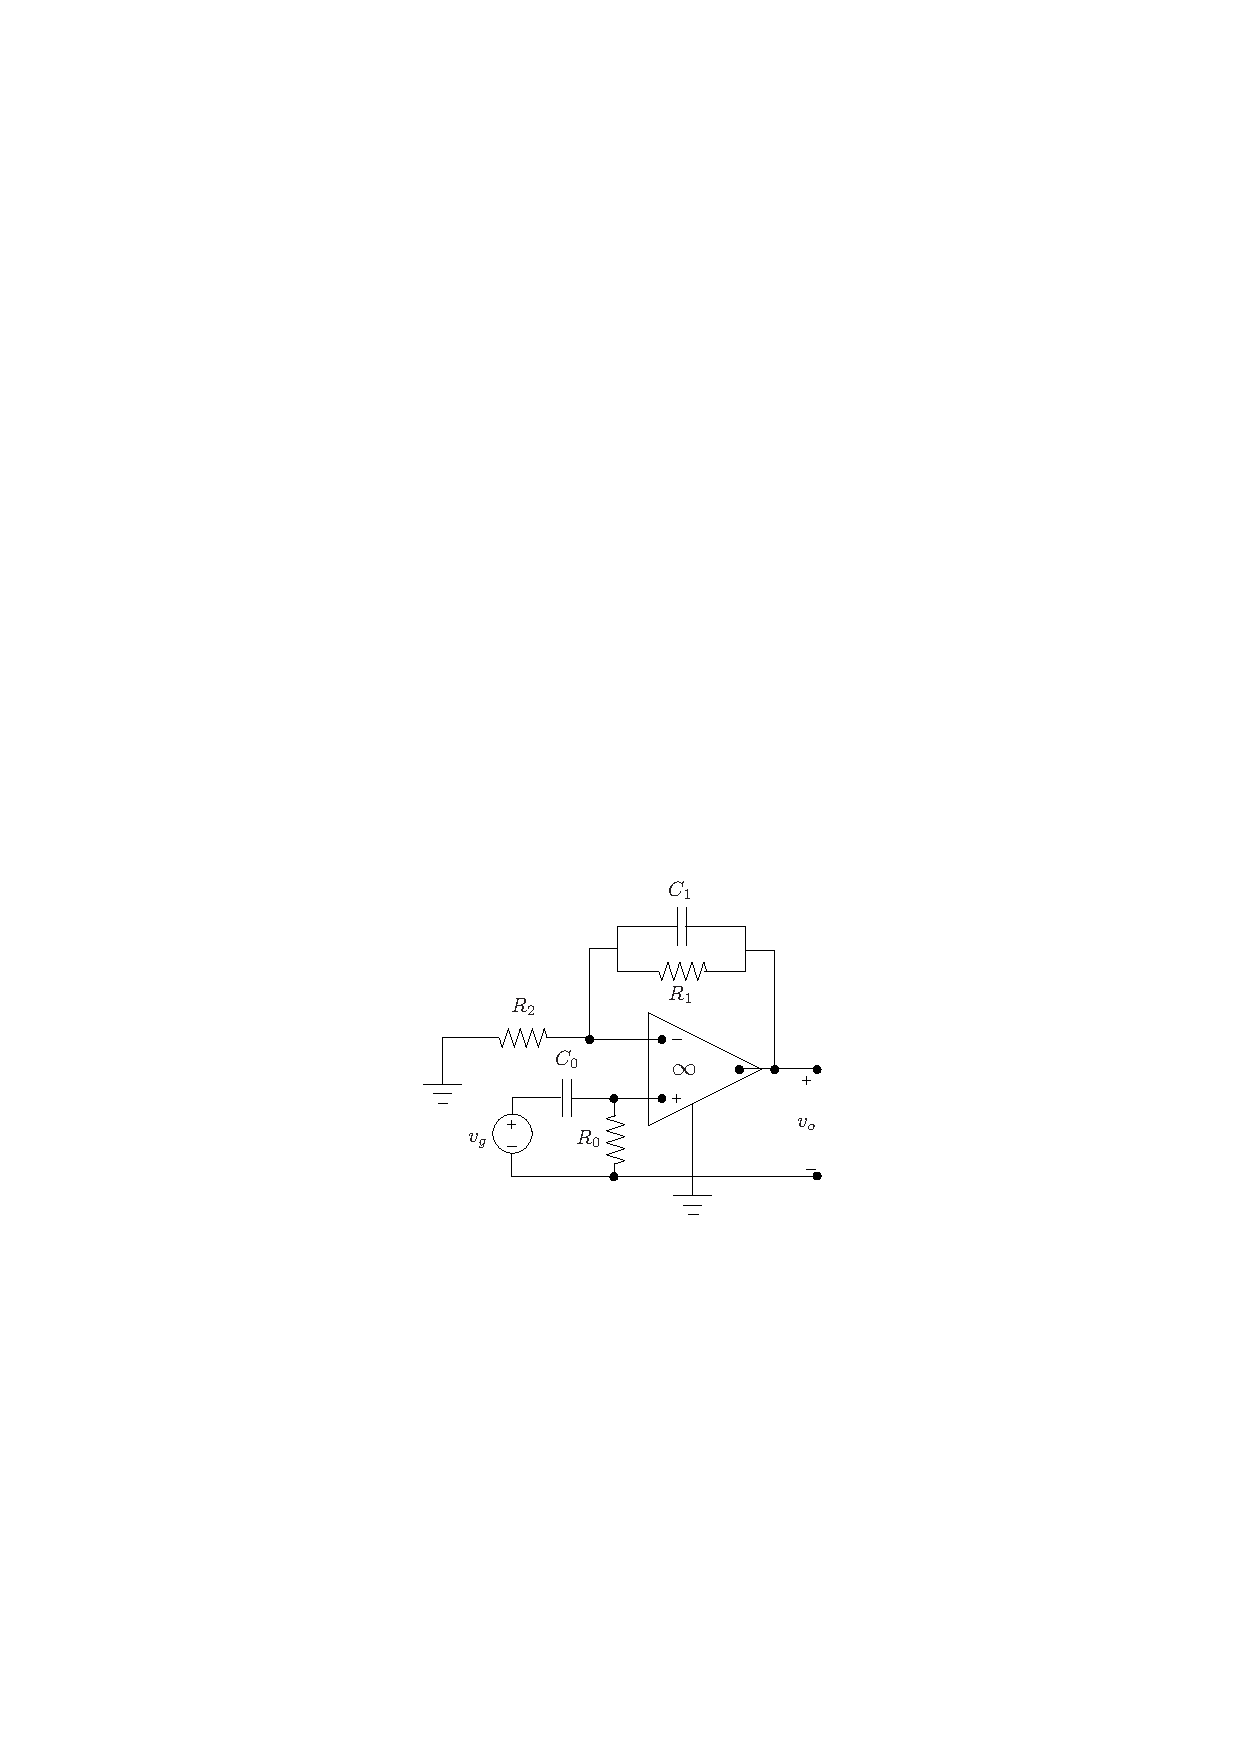
\includegraphics[width=0.6\textwidth]{exercices/ex-4-7}
\end{center}
avec 
\[R_0=1\,\,\mbox{k}\Omega \,\, , R_1=100\,\,\Omega \,\, , C_0=10\,\,\mu\mbox{F}\,\, , 
	C_1=1\,\,\mu\mbox{F}\,\, , R_2=10\,\,\mbox{k}\Omega \]

D�terminer
\begin{enumerate}
	\item la r�ponse fr�quentielle gain en tension � circuit ouvert:
	\[H(j\omega)=\left.\frac{\bar{V}_0}{\bar{V}_g}\right|_{\bar{I}_2=0}\]
	\item l'expression de $v_0(t)$ si $v_g(t)=2\cos 100 t$
\end{enumerate}

\rep{
	$H(j\omega)=  
	\frac{j\omega+ \frac{1}{R_1 C_1}+\frac{1}{R_2C_1}}
	{j\omega+\frac{1}{R_1 C_1}}\, . \, \frac{j\omega}{j\omega+\frac{1}{R_0 C_0}}$\\
	$v_0(t)=1.43 \cos (100 t +\frac{\pi}{4})$
}
\end{exercise}